To provide a more quantitative measure of the difference between the moist baroclinic wave simulations, the l\textsubscript{2} difference norm of p\textsubscript{s} between two simulations is computed as the time varying global integral in spherical coordinates:

\begin{equation} \label{}
l_2\big(\,p_s(t)\,\big) =& \Bigg[ \frac{1}{4\pi}\int^{2\pi}_{0} \int^{\frac{\pi}{2}}_{-\frac{\pi}{2}} \ \Big(\,p_{s_1}(\lambda,\varphi,t) - p_{s_0}(\lambda,\varphi,t)\,\Big)^2 \, cos(\varphi) \, d\varphi \, d\lambda\\\ \Bigg]^\frac{1}{2}.
\end{equation}

The l\textsubscript{2} difference norm between CAM-SE and CAM-HOMME is shown in \ref{fig:l2norm} for the $1^{\circ}$ and $\frac{1}{4}^{\circ}$ resolution simulations. The l\textsubscript{2} norms for the $1^{\circ}$ and $\frac{1}{4}^{\circ}$ have similar time varying magnitudes. As the baroclinic waves evolve, the l\textsubscript{2} norms grow to a maximum on the order of 1 hPa by day 15 (\ref{fig:l2norm}). To assess the significance of the l\textsubscript{2} norms, an l\textsubscript{2} norm that serves as an estimate of the uncertainty of a high resolution reference simulation is computed after (Jablonowski and Williamson 2006). The uncertainty in the reference is taken as the l\textsubscript{2} between a pair of $\frac{1}{4}^{\circ}$ resolution moist baroclinic wave simulations using different dynamical cores, CAM-SE and CAM-FV. At a $\frac{1}{4}^{\circ}$ resolution, the moist baroclinic wave solutions are converged to within a tolerable level of error (not shown), and therefore comparison between dynamical cores serves as an estimate of the uncertainty in the reference solutions arising from model imperfections. 

The black curve in \ref{fig:l2norm} is the l\textsubscript{2} difference norm between CAM-SE and CAM-FV at approximately a $\frac{1}{4}^{\circ}$ resolution. l\textsubscript{2} values that fall below the uncertainty in the reference are considered insignificant. The l\textsubscript{2} between CAM-SE and CAM-HOMME generally lie near or below the uncertainty in the reference solution, indicating the differences between CAM-SE and CAM-HOMME are insignificant for the case of the moist baroclinic wave. This is consistent with the corresponding time varying, global minimum in p\textsubscript{s} for all the simulations, which illustrates that the differences between CAM-SE and CAM-HOMME are smaller than the differences arising from increasing the horizontal resolution (\ref{fig:l2norm}).

\begin{figure}[x]
\centering
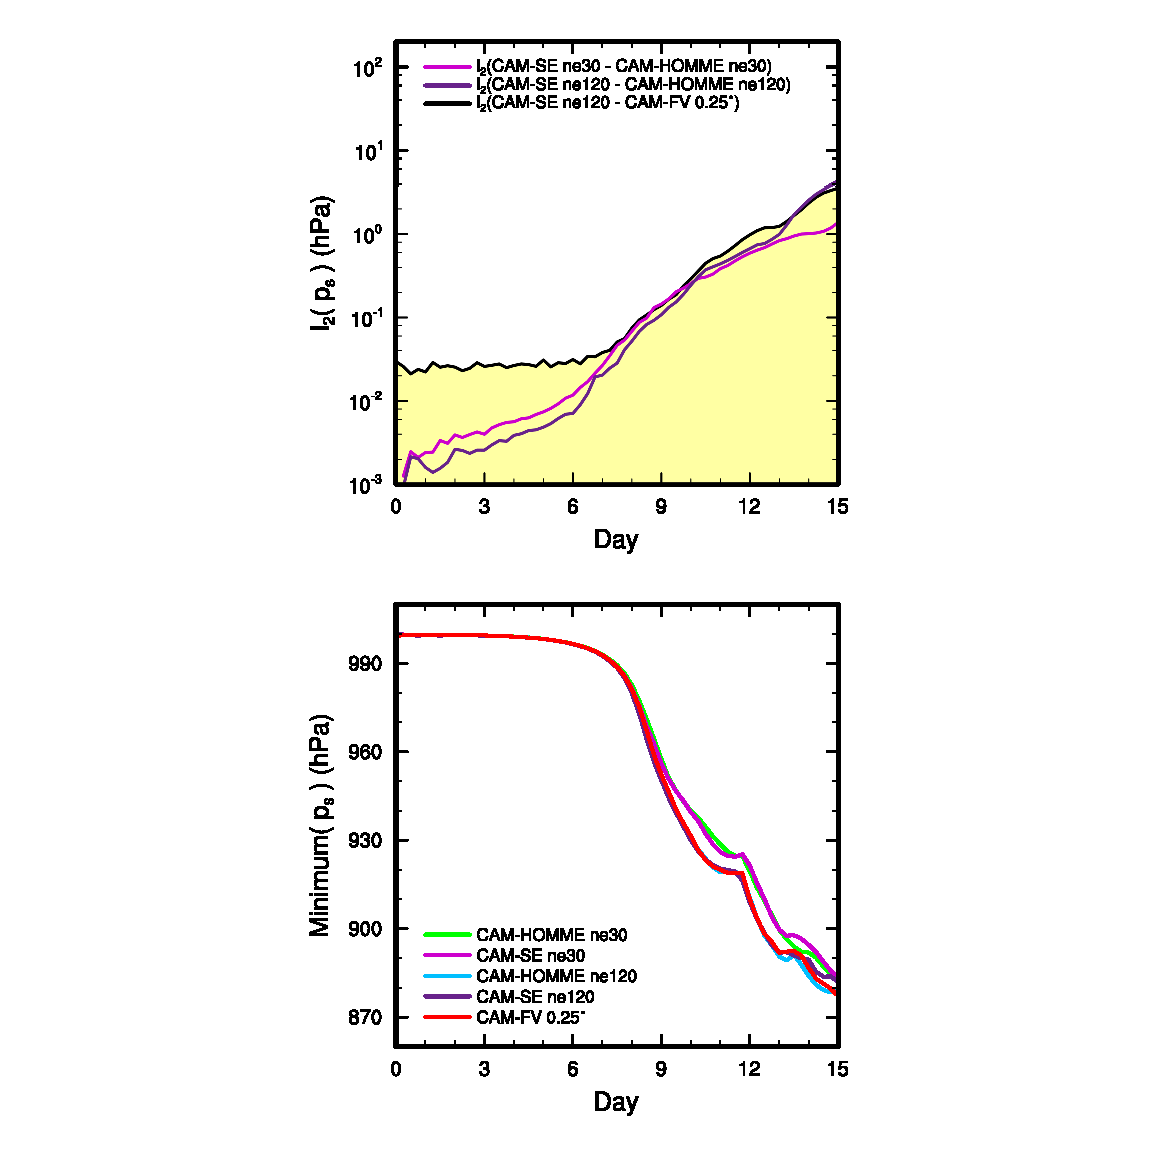
\includegraphics[width=20pc]{figs/temp_l2_reference.eps}
\caption{(Upper) l\textsubscript{2} difference norms of p\textsubscript{s} in the moist baroclinic wave simulations. l\textsubscript{2} values lying within the yellow region fall below the estimate of the uncertainty in the reference solution (black curve). (lower) Global minimum p\textsubscript{s} in the moist baroclinic wave simulations.}
\label{fig:l2norm}
\end{figure}
